\documentclass{article}
\usepackage{tikz}
\usetikzlibrary{matrix,chains,positioning,decorations.pathreplacing,arrows}

\begin{document}

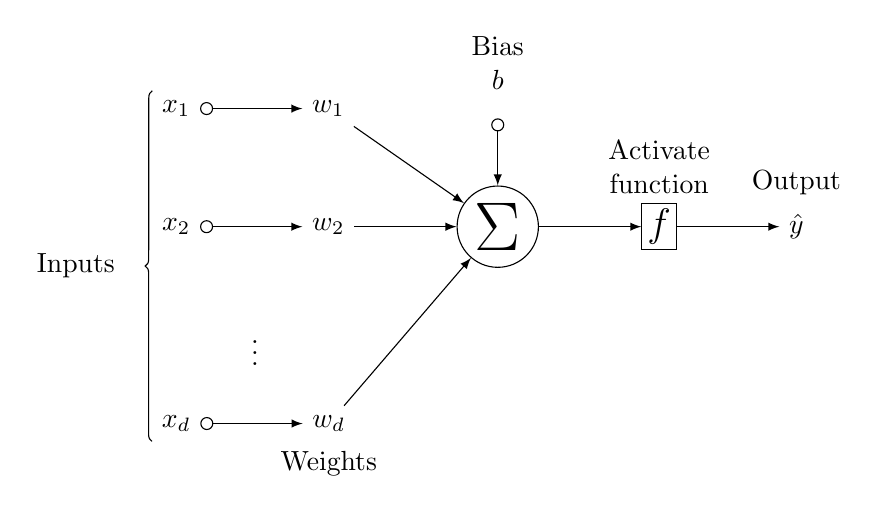
\begin{tikzpicture}[
init/.style={
  draw,
  circle,
  inner sep=2pt,
  font=\Huge,
  join = by -latex
},
squa/.style={
  draw,
  inner sep=2pt,
  font=\Large,
  join = by -latex
},
start chain=2,node distance=13mm
]
\node[on chain=2] 
  (x2) {$x_2$};
\node[on chain=2,join=by o-latex] 
  {$w_2$};
\node[on chain=2,init] (sigma) 
  {$\displaystyle\Sigma$};
\node[on chain=2,squa,label=above:{\parbox{2cm}{\centering Activate \\ function}}]   
  {$f$};
\node[on chain=2,label=above:Output,join=by -latex] 
  {$\hat{y}$};
\begin{scope}[start chain=1]
    \node[on chain=1] at (0,1.5cm) 
    (x1) {$x_1$};
    \node[on chain=1,join=by o-latex] 
      (w1) {$w_1$};
\end{scope}

\begin{scope}[start chain=3]
\node[on chain=3] at (1,-1.5cm) 
 {$\vdots$};
\end{scope}

\begin{scope}[start chain=4]
\node[on chain=4] at (0,-2.5cm) 
  (xd) {$x_d$};
\node[on chain=4,label=below:Weights,join=by o-latex] 
  (wd) {$w_d$};
\end{scope}

\node[label=above:\parbox{2cm}{\centering Bias \\ $b$}] at (sigma|-w1) (b) {};

\draw[-latex] (w1) -- (sigma);
\draw[-latex] (wd) -- (sigma);
\draw[o-latex] (b) -- (sigma);

\draw[decorate,decoration={brace,mirror}] (x1.north west) -- node[left=10pt] {Inputs} (xd.south west);
\end{tikzpicture}

\end{document}
